% Figure snippets for scRareRefine Bioinformatics-style draft v2.

\begin{figure}[t]
\centering
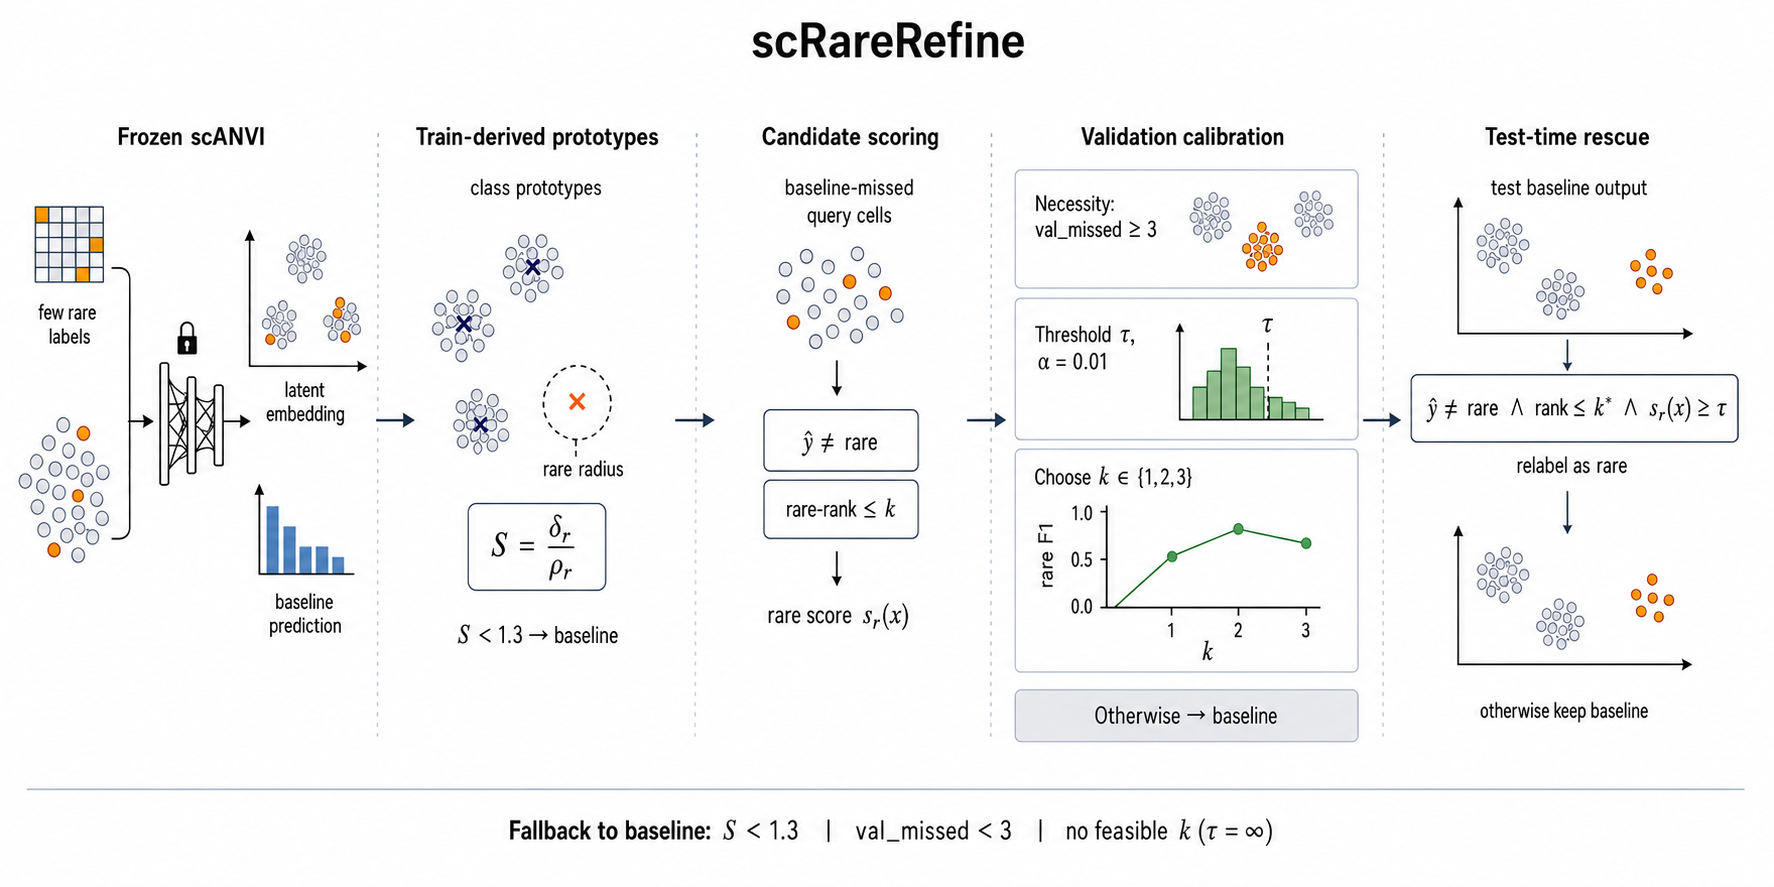
\includegraphics[width=\linewidth]{fig1_overview.png}
\caption{\method\ workflow. scANVI provides latent embeddings and initial predictions; \method\ fits train-only prototypes, selects validation-only gates and conformal thresholds, and evaluates rescue on held-out test cells.}
\label{fig:overview}
\end{figure}

\begin{figure}[t]
\centering
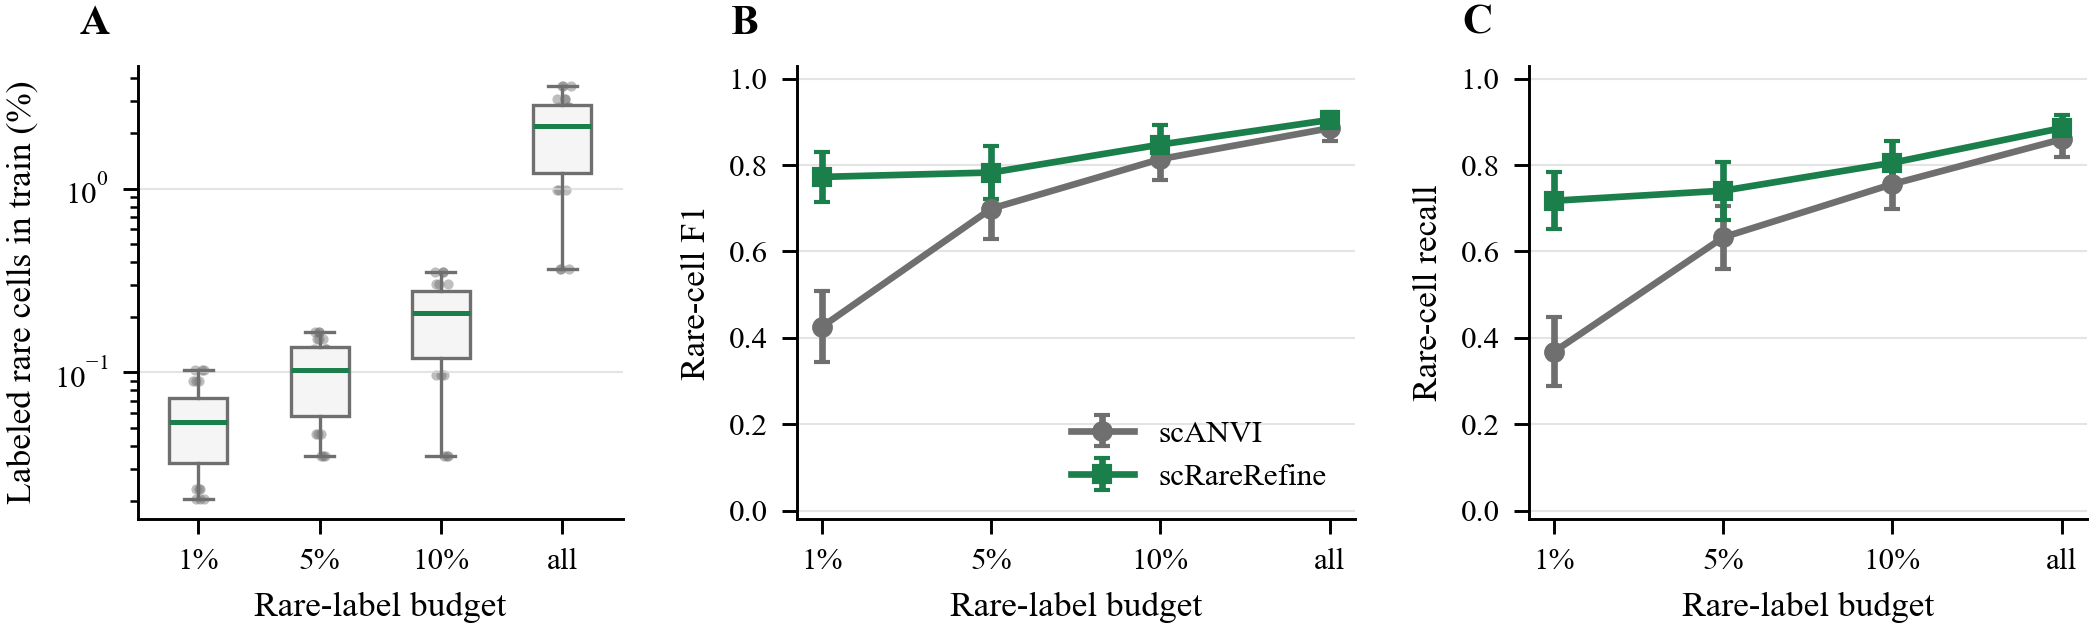
\includegraphics[width=\linewidth]{fig2_label_scarcity_recovery.pdf}
\caption{Rare-label scarcity and recovery across label budgets. (A) Labeled rare cells as a percentage of all training cells. (B,C) Mean rare-cell F1 and recall for scANVI and \method\ across eight datasets and three seeds; error bars show standard errors over run-level units.}
\label{fig:scarcity-recovery}
\end{figure}

\begin{figure}[t]
\centering
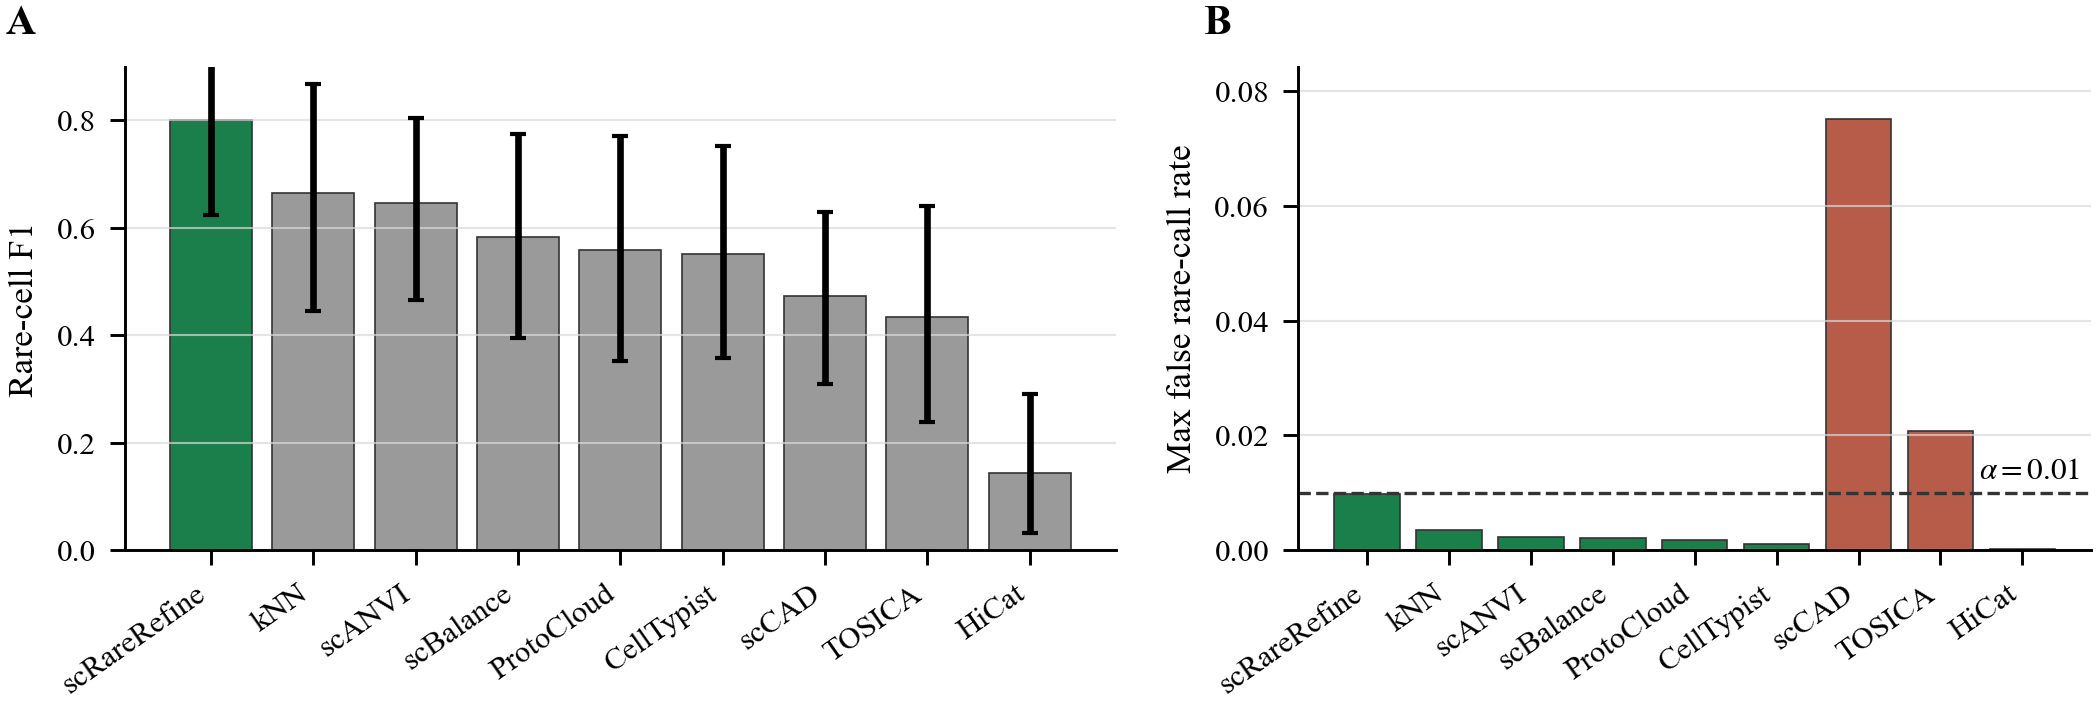
\includegraphics[width=\linewidth]{fig3_scarce_benchmark.pdf}
\caption{Scarce-label benchmark summary. (A) Mean rare-cell F1 with bootstrap 95\% confidence intervals over run-level units. (B) Maximum false rare-call rate in the same scarce-label region; the dashed line marks the pre-specified $\alpha=0.01$ budget.}
\label{fig:scarce-benchmark}
\end{figure}

\begin{figure}[t]
\centering
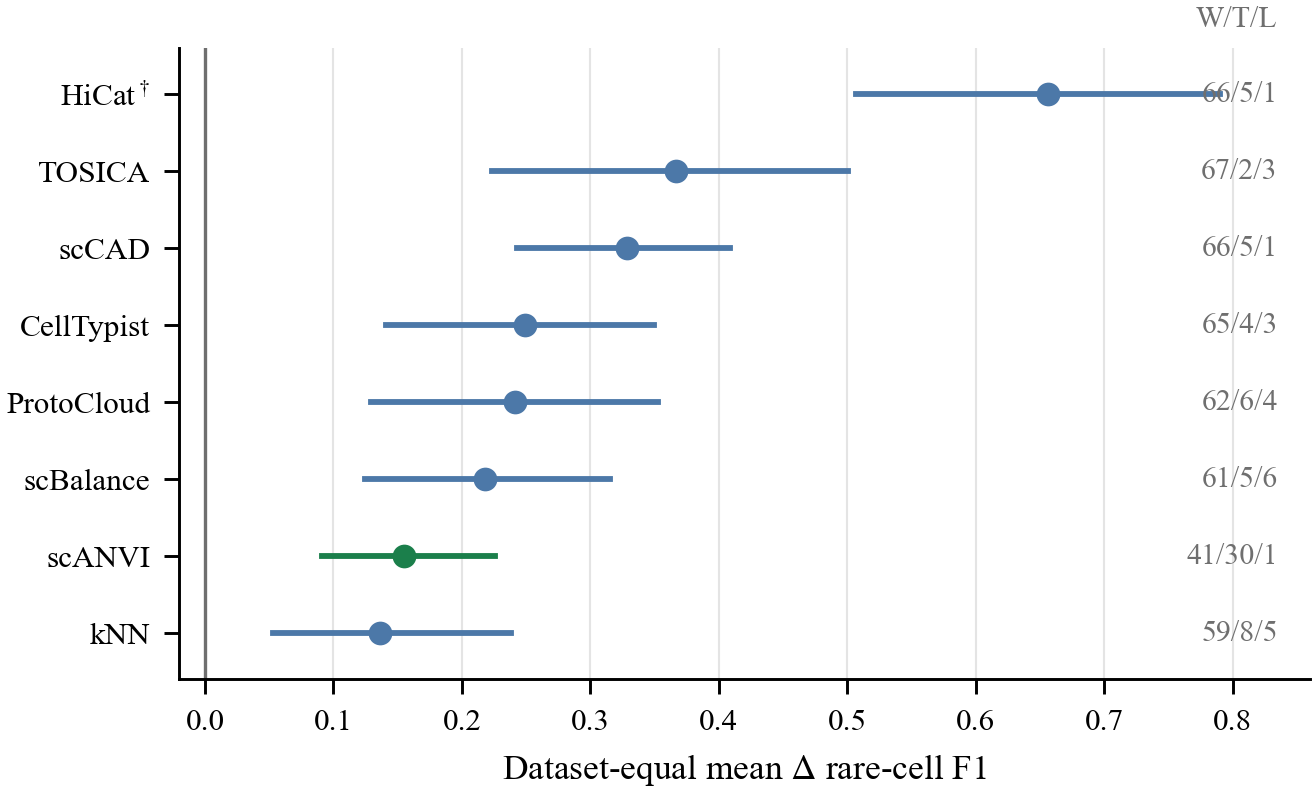
\includegraphics[width=0.72\linewidth]{fig4_paired_delta_forest.pdf}
\caption{Paired rare-F1 improvements in the scarce-label region. Points show mean paired $\Delta$F1 for \method\ minus each comparator; horizontal intervals are bootstrap 95\% confidence intervals. Win/tie/loss counts are shown at right.}
\label{fig:paired-delta}
\end{figure}
